\documentclass[12pt]{report}

\usepackage[english]{babel}
\usepackage[utf8x]{inputenc}
\usepackage{amsmath}
\usepackage{graphicx}
\usepackage{multirow}
\usepackage[hypcap]{caption}
\usepackage{setspace} 
\usepackage{float}

\title{Lab 5: High Temperature Creep and Creep Rupture}
\author{Zachary Tschirhart \\
	\small \\
        \small EID: zst75 \\
	\small Department of Aerospace Engineering and Engineering Mechanics \\
	\small \textbf{ASE 324L (Mon 2:00-5:00)} \\
	\small Unique: 13740}

\date{February 27, 2014}


\begin{document}
\maketitle

\setcounter{secnumdepth}{0}

\section{Results and Discussion}
\doublespacing

\subsection{Question 1a}

\begin{figure}[H]
	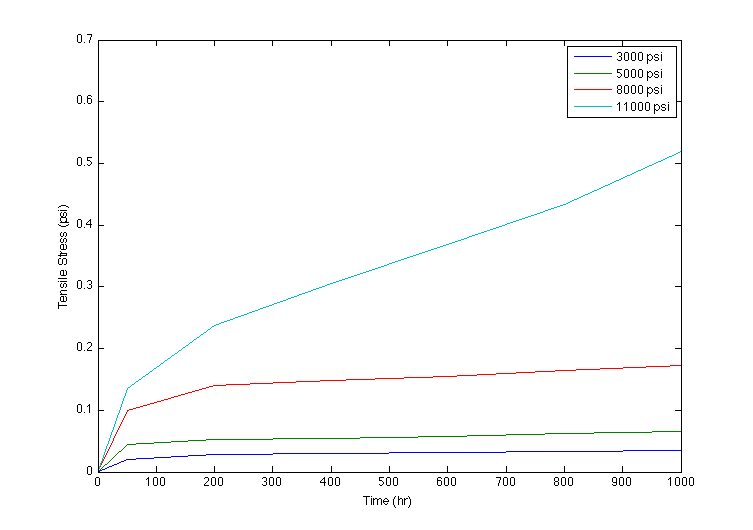
\includegraphics[width=1\textwidth]{problem1a.png}
	\caption{Creep curve for each different Tensile Stress}
	\label{fig:Figure1}
\end{figure}

\subsection{Question 1b}

Using MATLAB to find delta time as mean(diff([400 600 800 1000])) and similarlly for each tensile stress group. When this was found, delta \(\epsilon\) for each was divided by delta time.
\\
\(\dot{\epsilon_{3000}}\) = 8.75e-6 \\
\(\dot{\epsilon_{5000}}\) = 1.50e-5 \\
\(\dot{\epsilon_{8000}}\) = 4.13e-5 \\
\(\dot{\epsilon_{11000}}\) = 3.53e-4 \\

\subsection{Question 1c}
When doing a linear fit on the log-log plot, this gives the n and B values.

\begin{figure}[H]
	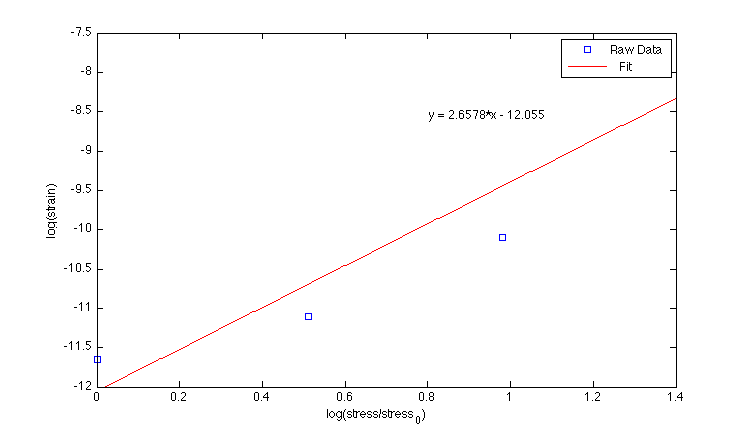
\includegraphics[width=1\textwidth]{problem1c.png}
	\caption{Curve fitting to get n and B for power law}
	\label{fig:Figure2}
\end{figure}

n = 2.6578 \\
B = exp(-12.055) = 5.815e-6

\subsection{Question 2a}

\begin{figure}[H]
	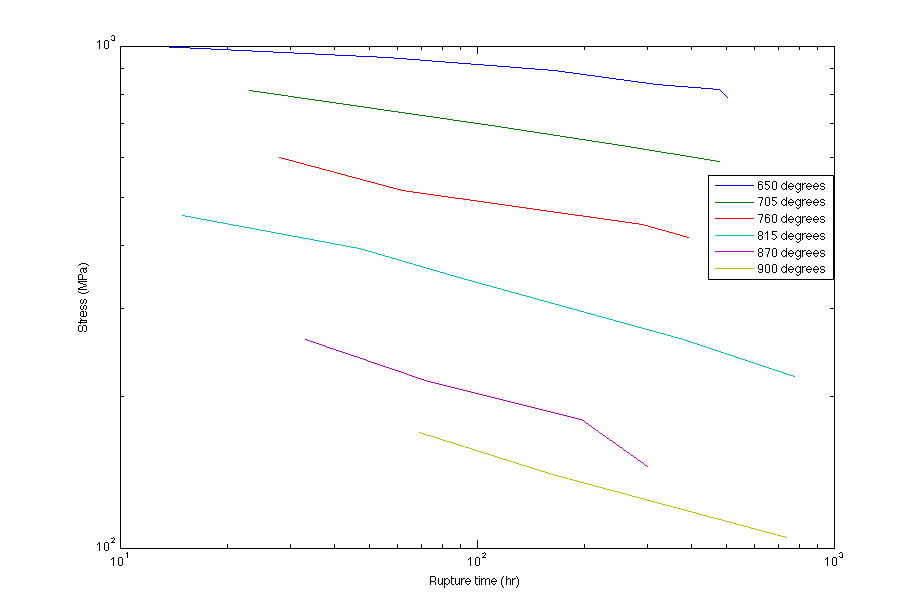
\includegraphics[width=1\textwidth]{problem2a.png}
	\caption{Stress vs. Rupture Time}
	\label{fig:Figure3}
\end{figure}

\subsection{Question 2b}

\begin{figure}[H]
	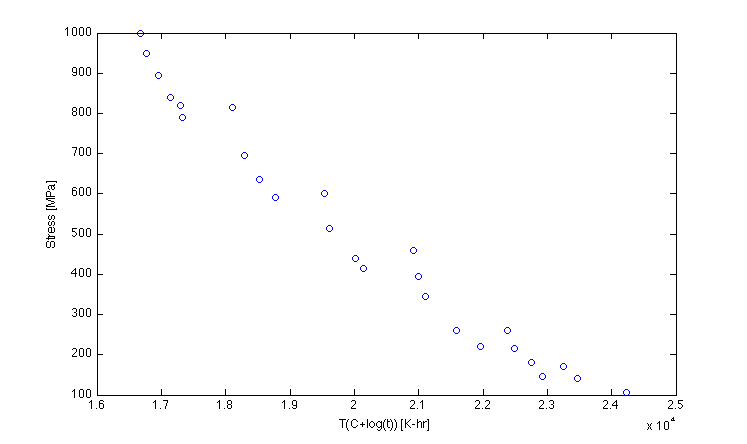
\includegraphics[width=1\textwidth]{problem2b.png}
	\caption{Larson-Miller plot}
	\label{fig:Figure4}
\end{figure}

\subsection{Question 2c}
This is just a problem of getting the Larson-Miller value at 260 MPa, which is 21.58e3.

\begin{equation}
  log(t_R) = \frac{21.58x10^3}{600} - 20 = 15.966 hr
  \label{equation:equation1}
\end{equation}

The final time is \(t_R\) = 9.26e15 hours

\subsection{Question 2d}
There would be no additional information needed to determine a course C value, since this can be determined by two sets of rupture time and temperature data for a material at the same measured stress, then using equation 6 from the lab manual. If we wanted a better approximation of C, then more measurements would need to be taken at the same stresses with temperature varied. 

\subsection{Question 3}
Hand-written

\subsection{Question 4}
Firstly, all of the variables need to be identified: B = \(10^{-26}\), n = 5, \(\sigma_0\) = 4000 psi, and E = \(30x10^{6}\) psi. Then the equation 1/\(\sigma^n_0\) = -BE needs to be integrated then the solved for t.

t = 21932 hours

\subsection{Question 5}

Elasticity, is just the linear portion of the stress-strain curve. There is no permanent deformations until the yield stress is reached. 

Dislocation glide is when the dislocations keep their original length in the lattice structure. This creep happens at high stresses and doesn't matter what temperature (mostly). 

Dislocation creep is much like dislocation glide, where atoms diffuse into or out of the dislocation core, leading to dislocation climb. The dislocation climb-and-glide leads to creep.

Coble creep happens at relatively low temperature and grain-boundary diffusion dominates bulk diffusion. The creep has an inverse relationship with the grain size cubed.

N-H creep, is when stress drives bulk diffusion within grains. This happens at low stress but high temperature. The creep has an inverse relationship with the grain size squared.

\end{document}
